%% Manuscript for the International Journal of Information Technology (Springer Nature, BVICAM).
%% Springer Nature LaTeX template (sn-jnl), Math and Physical Sciences numbered reference style.
\documentclass[pdflatex,sn-mathphys-num]{sn-jnl}

\usepackage{graphicx}
\usepackage{multirow}
\usepackage{amsmath,amssymb,amsfonts}
\usepackage{amsthm}
\usepackage{xcolor}
\usepackage{textcomp}
\usepackage{booktabs}
\usepackage{array}
\usepackage{algorithm}
\usepackage{algpseudocode}
\usepackage{tikz}
\usetikzlibrary{arrows.meta,positioning,fit}

\raggedbottom

% The bibliography style wraps DOIs as \def\doiurl#1{\url{...#1}}, which reads
% the argument before \url can neutralize "_" and drops underscores. Read the
% argument with "_" as a plain character instead.
\makeatletter
\newcommand{\doiurl}{\begingroup\catcode`\_=12\relax\doiurl@}
\newcommand{\doiurl@}[1]{\endgroup\url{https://doi.org/#1}}
\makeatother
% Repository link, defined with "_" as a plain character so it survives anywhere.
\begingroup\catcode`\_=12
\gdef\repourl{\url{https://github.com/Arc-001/twin_turbo}}
\endgroup

\begin{document}

\title[Hybrid edge intelligence and digital twins for turbofan maintenance]{Twin Turbo: calibrated hybrid edge intelligence and particle-filter digital twins for autonomous turbofan maintenance decisions}

\author*[1]{\fnm{Archit} \sur{Singh}}\email{architsingh24@gmail.com}
\author[1]{\fnm{Vedant} \sur{Vadke}}\email{vadkevedant07@gmail.com}
\author[1]{\fnm{Rishabh} \sur{Raushan}}\email{rishabhraushan200524@gmail.com}
\author[1]{\fnm{Sreevarsh Mahesh} \sur{Gandhi}}\email{sreevarshmaheshgandhi@gmail.com}

\affil*[1]{\orgdiv{Department of Computer Science and Engineering (AI/ML)}, \orgname{SRM Institute of Science and Technology}, \orgaddress{\city{Kattankulathur, Chennai}, \postcode{603203}, \state{Tamil Nadu}, \country{India}}}

\abstract{Remaining-useful-life (RUL) models for turbofan engines are usually judged by point-prediction error at one truncated cycle, which says little about whether the maintenance decisions they drive are safe. This paper presents Twin Turbo, a hybrid framework in which a lightweight edge model runs every cycle and a per-engine digital twin is consulted only when needed. The edge model is a gradient-boosted regressor wrapped in Mondrian conformal prediction; the twin is a particle filter over an exponential health-index degradation model with a fleet-learned prior. The edge model synchronizes the twin when a trigger fires, and the policy acts on the more cautious of the two calibrated lower bounds. On the NASA C-MAPSS test sets the twin attains RMSE of 10.33--14.78, and its 90\% intervals reach 86--94\% coverage, against 43--54\% for Monte-Carlo dropout on an LSTM. Replaying 709 held-out engines from first cycle to failure, the hybrid policy lets no engine fail, lowers long-run maintenance cost by 34--47\% relative to optimal age replacement, and consults the twin on 21--28\% of cycles. It is the only policy evaluated that remains failure-free at every grounding threshold, including with no safety margin.}

\keywords{Predictive maintenance, Remaining useful life, Digital twin, Particle filter, Conformal prediction, Edge computing}

\maketitle

%% ===================================================================== 1
\section{Introduction}\label{sec:intro}

Maintenance is a large share of the operating cost of aircraft engines, and its central decision is when an engine should come off the wing. Removing it too late risks an unplanned in-service failure, the most expensive and most dangerous outcome. Removing it too early discards flight cycles that were already paid for. Time-based maintenance retires every unit at a fixed age chosen from fleet lifetime statistics~\cite{barlow1960optimum}; it is safe on average but wasteful, because it treats the longest-lived engine exactly like the shortest-lived one. Condition-based maintenance instead uses each engine's own sensor data to estimate its remaining useful life (RUL) and act on it~\cite{jardine2006review,lei2018review}.

The NASA C-MAPSS dataset~\cite{saxena2008damage}, which simulates fleets of turbofans degrading from a healthy state to failure under noise, multiple operating regimes and multiple fault modes, is the standard benchmark for RUL estimation~\cite{ramasso2014benchmark}. Reported accuracy on it has improved steadily through convolutional~\cite{babu2016cnn,li2018dcnn}, recurrent~\cite{zheng2017lstm}, hybrid~\cite{aldulaimi2019hdnn} and attention-based~\cite{ragab2020ats2s} networks. Three gaps nevertheless separate these models from an autonomous maintenance system.

First, point estimates are not decisions. A prediction of 40 remaining cycles with an error of $\pm5$ supports a very different action from the same prediction with an error of $\pm40$. Most published C-MAPSS models output a single number; where uncertainty is added, typically through Monte-Carlo (MC) dropout~\cite{gal2016dropout}, its calibration is rarely checked, and benchmarks show that calibration quality varies widely across methods~\cite{basora2023uqbench}. Second, accuracy is measured in the wrong place. The benchmark protocol scores each test engine only at the last cycle of a truncated trajectory, which reveals nothing about whether a policy built on the model would ground engines in time or what it would cost relative to retiring engines at a fixed age. Third, ``digital twin'' is used loosely. As articulated by Glaessgen and Stargel~\cite{glaessgen2012digital} and formalized by Grieves and Vickers~\cite{grieves2017digital}, a twin is a virtual model bound to one specific physical asset and kept synchronized with it; fleet-trained neural regressors hold no per-asset state, yet are frequently presented as twins.

Deployment also imposes a systems constraint. A model that runs on or near the engine every cycle must be small and stateless, while a model that maintains a detailed belief about each engine is naturally hosted off board, where consulting it costs communication. Edge computing~\cite{shi2016edge} and cascaded inference~\cite{teerapittayanon2016branchynet} suggest the pattern of running a cheap model always and escalating to an expensive one only when needed.

This paper presents Twin Turbo, a framework that addresses the three gaps within that edge/twin pattern. A gradient-boosted edge model runs every cycle and is wrapped in Mondrian conformal prediction~\cite{vovk2005alrw,angelopoulos2021gentle}, which gives it calibrated intervals at negligible cost. A digital twin, instantiated once per engine, tracks a sensor-fused health index~\cite{wang2008similarity} with a particle filter~\cite{arulampalam2002tutorial,orchard2009particle} over an exponential degradation model whose population prior is learned from run-to-failure engines~\cite{gebraeel2005residual}. The twin is synchronized only when the edge model raises a trigger, and a fixed policy maps the more cautious of the two calibrated lower bounds to one of four actions. The contributions are:
\begin{enumerate}
\item An instance-specific, synchronizable digital twin for turbofan prognostics that combines a learned health index with Bayesian particle filtering of a fleet prior, and whose 90\% posterior intervals are empirically calibrated without tuning.
\item A hybrid edge/twin decision architecture with conformally calibrated edge intervals, trigger-based twin synchronization, and a cautious fusion rule that preserves at least 90\% coverage by the union bound.
\item A decision-level evaluation protocol that replays 709 held-out engines from first cycle to failure and scores every policy by failures, unused life and renewal-reward cost rate against optimal age replacement~\cite{barlow1960optimum}, edge-only, twin-only, LSTM and oracle baselines, with ablations of each design choice.
\item An open, reproducible implementation (\repourl) in which every table and figure is regenerated from cached per-cycle traces.
\end{enumerate}

Section~\ref{sec:related} reviews related work. Section~\ref{sec:data} describes the dataset and preprocessing, and Section~\ref{sec:method} the edge model, digital twin and decision layer. Section~\ref{sec:protocol} gives the experimental protocol, Section~\ref{sec:results} the results and ablations, and Section~\ref{sec:discussion} discusses limitations before Section~\ref{sec:conclusion} concludes.

%% ===================================================================== 2
\section{Related work}\label{sec:related}

\subsection{Prognostics and the C-MAPSS benchmark}
Prognostics estimates the RUL of an asset from condition-monitoring data so that maintenance can be planned before failure~\cite{jardine2006review,lei2018review}. Approaches are usually grouped into physics-based, statistical and machine-learning models~\cite{si2011review,lei2018review}. C-MAPSS~\cite{saxena2008damage} was released by NASA for the 2008 PHM data challenge and remains the most widely used RUL benchmark; Ramasso and Saxena~\cite{ramasso2014benchmark} surveyed the methods applied to it and documented inconsistencies in how results are reported, including RUL clipping and evaluation protocol.

\subsection{Statistical and model-based prognostics}
Two strands of this literature shape our digital twin. For health-index (HI) construction, Wang et al.~\cite{wang2008similarity}, a winning approach at PHM08, fuse sensors into one HI by regressing sensor values onto 1 for early-life and 0 for end-of-life cycles. For stochastic degradation with Bayesian updating, Gebraeel et al.~\cite{gebraeel2005residual} model degradation as an exponential process whose parameters have a population prior learned from a fleet, and update that prior with each observation of the individual unit to obtain a residual-life distribution. Particle filters~\cite{arulampalam2002tutorial} generalize this updating to nonlinear, non-Gaussian settings; Orchard and Vachtsevanos~\cite{orchard2009particle} established particle filtering for online failure prognosis, and the Liu--West kernel-shrinkage scheme~\cite{liu2001combined} is the standard way to estimate static parameters inside a particle filter without particle collapse. Such models are interpretable and yield full predictive distributions, but are seldom benchmarked against deep models on C-MAPSS.

\subsection{Deep learning for RUL}
Since 2016, deep networks trained on sliding windows of raw sensor data have dominated reported C-MAPSS accuracy. Babu et al.~\cite{babu2016cnn} introduced convolutional networks for RUL regression, Zheng et al.~\cite{zheng2017lstm} applied LSTMs~\cite{hochreiter1997lstm}, and Li et al.~\cite{li2018dcnn} showed that deeper 1-D convolutions with a piecewise-linear target reach RMSE near 12.6 on FD001. Later work added semi-supervised pre-training~\cite{listou2019semisup}, encoder--decoders~\cite{yu2019bilstmed}, hybrid CNN--LSTM architectures~\cite{aldulaimi2019hdnn} and attention~\cite{ragab2020ats2s}. Table~\ref{tab:literature} compiles representative results. Gradient-boosted trees~\cite{friedman2001gbm,ke2017lightgbm} on hand-crafted window features remain a strong and far cheaper baseline. Across this line of work, models output a point estimate without calibrated confidence, and accuracy is reported only at the last observed cycle of each truncated test engine.

\begin{table}[t]
\caption{Published test-set RMSE on C-MAPSS for representative methods, as compiled by Ragab et al.~\cite{ragab2020ats2s}. Lower is better.}\label{tab:literature}
\begin{tabular*}{\textwidth}{@{\extracolsep\fill}lcccc}
\toprule
Method & FD001 & FD002 & FD003 & FD004 \\
\midrule
Gradient boosting~\cite{zhang2016modbne}  & 15.67 & 29.09 & 16.84 & 29.01 \\
2-D CNN~\cite{babu2016cnn}               & 18.45 & 30.29 & 19.82 & 29.16 \\
Deep LSTM~\cite{zheng2017lstm}           & 16.14 & 24.49 & 16.81 & 28.17 \\
1-D deep CNN~\cite{li2018dcnn}           & 12.61 & 22.36 & 12.64 & 23.31 \\
MODBNE ensemble~\cite{zhang2016modbne}   & 15.04 & 25.05 & 12.51 & 28.66 \\
BiLSTM encoder--decoder~\cite{yu2019bilstmed} & 14.74 & 22.07 & 17.48 & 23.49 \\
Hybrid DNN~\cite{aldulaimi2019hdnn}      & 13.02 & 15.24 & 12.22 & 18.16 \\
Attention seq2seq~\cite{ragab2020ats2s}  & 12.63 & 14.65 & 11.44 & 16.66 \\
\botrule
\end{tabular*}
\end{table}

\subsection{Uncertainty quantification}
MC dropout~\cite{gal2016dropout} and deep ensembles~\cite{lakshminarayanan2017ensembles} are the most common ways to attach uncertainty to neural RUL predictors, but their calibration is not guaranteed: Basora et al.~\cite{basora2023uqbench} find that it varies substantially across methods and engines. Conformal prediction~\cite{vovk2005alrw,angelopoulos2021gentle} wraps any point predictor and provides intervals with a finite-sample, distribution-free coverage guarantee under exchangeability. Mondrian (group-conditional) variants calibrate separately within bins, which matters for RUL because error grows with distance from failure.

\subsection{Digital twins and edge inference}
Glaessgen and Stargel~\cite{glaessgen2012digital} described the digital twin as a model that mirrors the life of its flying twin by combining physics, fleet history and the vehicle's own sensor data; Grieves and Vickers~\cite{grieves2017digital} formalized it as a virtual counterpart linked to one physical instance and kept synchronized with it, and Tao et al.~\cite{tao2019digital} review industrial uses, with prognostics among the most prominent. Two properties recur in these definitions: the model is instance-specific, and it is synchronized with its asset as data arrive. Edge computing places computation near data sources to reduce latency, bandwidth and dependence on connectivity~\cite{shi2016edge}, and cascaded or early-exit inference~\cite{teerapittayanon2016branchynet} defers to an expensive model only when a cheap one is not confident. We apply the same idea across a device/twin boundary.

\subsection{From predictions to maintenance decisions}
Classical reliability theory gives the baseline any predictive policy must beat: age replacement, which replaces a unit at the fixed age that minimizes the long-run cost rate of the renewal process~\cite{barlow1960optimum}. We score every policy with the same renewal-reward cost rate, so predictive maintenance is compared against the optimal time-based policy and not only against run-to-failure. Table~\ref{tab:gap} positions this work against the families above.

\begin{table}[t]
\caption{Typical properties of each family of approaches as applied to C-MAPSS, and of this work.}\label{tab:gap}
\begin{tabular*}{\textwidth}{@{\extracolsep\fill}>{\raggedright\arraybackslash}p{0.46\textwidth}ccc}
\toprule
Approach & \shortstack{Calibrated\\uncertainty} & \shortstack{Per-asset\\state} & \shortstack{Decisions\\evaluated} \\
\midrule
Similarity-based HI matching~\cite{wang2008similarity} & -- & -- & -- \\
Bayesian degradation / particle filters~\cite{gebraeel2005residual,orchard2009particle} & posterior & \checkmark & rarely \\
Deep point regressors~\cite{babu2016cnn,zheng2017lstm,li2018dcnn,ragab2020ats2s} & -- & -- & -- \\
Deep nets + MC dropout / ensembles~\cite{gal2016dropout,lakshminarayanan2017ensembles} & not guaranteed & -- & rarely \\
Conformal prediction~\cite{vovk2005alrw,angelopoulos2021gentle} & \checkmark & -- & rarely \\
Age replacement~\cite{barlow1960optimum} & n/a & -- & \checkmark \\
\midrule
This work & \checkmark & \checkmark & \checkmark \\
\botrule
\end{tabular*}
\end{table}

%% ===================================================================== 3
\section{Dataset and preprocessing}\label{sec:data}

C-MAPSS~\cite{saxena2008damage} contains four sub-datasets that vary difficulty on two axes: the number of operating regimes and the number of fault modes (Table~\ref{tab:data}). Each row is one engine at one flight cycle, with three operational settings and 21 sensor channels. Training trajectories run to failure; test trajectories are truncated at an arbitrary earlier cycle, and the ground-truth RUL at that cycle is provided separately and used only for scoring.

\begin{table}[t]
\caption{C-MAPSS sub-datasets. ``Features'' counts operational settings plus non-constant sensors retained after pruning.}\label{tab:data}
\begin{tabular*}{\textwidth}{@{\extracolsep\fill}lccccc}
\toprule
Dataset & Regimes & Fault modes & Train engines & Test engines & Features \\
\midrule
FD001 & 1 & 1 (HPC) & 100 & 100 & 18 \\
FD002 & 6 & 1 (HPC) & 260 & 259 & 24 \\
FD003 & 1 & 2 (HPC, fan) & 100 & 100 & 19 \\
FD004 & 6 & 2 (HPC, fan) & 249 & 248 & 24 \\
\botrule
\end{tabular*}
\end{table}

Preprocessing is fitted on training engines only, and inside cross-validation on the training folds only. Sensors whose standard deviation over the training set is below $10^{-5}$ are dropped. On FD002 and FD004, operating regimes are identified by $k$-means ($k=6$) on the three operational settings, and every feature is standardized with the mean and standard deviation of its own regime; on FD001 and FD003 a single global standardization is used. The training target is the piecewise-linear RUL $\min(T_i - t,\,125)$, where $T_i$ is the failure cycle of engine $i$, following common practice~\cite{li2018dcnn}; decision evaluation always uses the unclipped true RUL. Inputs are sliding windows of $W = 30$ cycles; windows at the start of life are left-padded by repeating the first row.

%% ===================================================================== 4
\section{Methodology}\label{sec:method}

Fig.~\ref{fig:arch} shows the architecture. The edge model produces an estimate and a conformal interval at every cycle, and also projects the current sensor vector onto a scalar health index that is buffered locally. When a trigger fires, the buffer is sent to the engine's digital twin, which assimilates it and returns a RUL posterior. The decision policy acts on a calibrated lower bound from whichever source is current.

\begin{figure}[t]
\centering
\resizebox{\textwidth}{!}{%
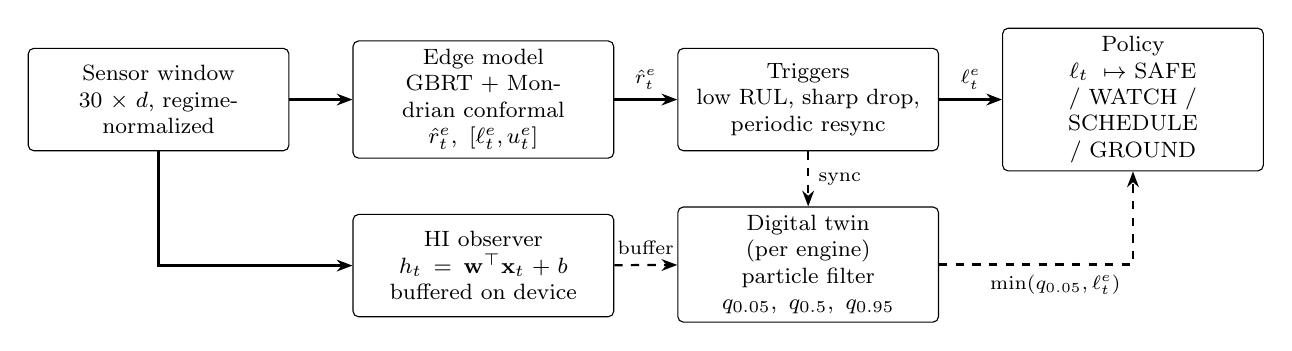
\begin{tikzpicture}[
  node distance=7mm and 8mm,
  box/.style={draw, rounded corners=2pt, align=center, font=\footnotesize, text width=31mm, minimum height=13mm, inner sep=3pt},
  arr/.style={-{Stealth[length=2mm]}, thick},
  lazy/.style={-{Stealth[length=2mm]}, thick, dashed},
  lab/.style={font=\scriptsize}]
\node[box] (win) {Sensor window\\$30\times d$, regime-normalized};
\node[box, right=of win] (edge) {Edge model\\GBRT + Mondrian conformal\\$\hat r^{e}_t,\ [\ell^{e}_t, u^{e}_t]$};
\node[box, right=of edge] (trig) {Triggers\\low RUL, sharp drop,\\periodic resync};
\node[box, right=of trig] (pol) {Policy\\$\ell_t \mapsto$ SAFE / WATCH /\\SCHEDULE / GROUND};
\node[box, below=of edge] (hi) {HI observer\\$h_t = \mathbf{w}^\top \mathbf{x}_t + b$\\buffered on device};
\node[box, below=of trig] (twin) {Digital twin (per engine)\\particle filter\\$q_{0.05},\ q_{0.5},\ q_{0.95}$};
\draw[arr] (win) -- (edge);
\draw[arr] (win.south) |- (hi.west);
\draw[arr] (edge) -- node[above, lab]{$\hat r^{e}_t$} (trig);
\draw[arr] (trig) -- node[above, lab]{$\ell^{e}_t$} (pol);
\draw[lazy] (trig) -- node[right, lab]{sync} (twin);
\draw[lazy] (hi) -- node[above, lab]{buffer} (twin);
\draw[lazy] (twin.east) -| node[pos=0.3, below, lab]{$\min(q_{0.05}, \ell^{e}_t)$} (pol.south);
\end{tikzpicture}}
\caption{Twin Turbo architecture. Solid arrows run every cycle on the edge; dashed arrows run only when a trigger fires.}\label{fig:arch}
\end{figure}

\subsection{Edge model with conformal intervals}\label{sec:edge}
Each window $X_t \in \mathbb{R}^{W\times d}$ is summarized per channel by its last value, mean, standard deviation and least-squares slope, giving a $4d$-dimensional vector (72--96 features). A histogram gradient-boosted regression tree ensemble~\cite{friedman2001gbm,pedregosa2011sklearn} with 150 trees of depth at most 6 and learning rate 0.08 maps this vector to a point estimate $\hat r^{e}_t$.

To calibrate it, out-of-fold predictions are obtained with five-fold cross-validation grouped by engine, and the deployed model is refit on all training engines. Residuals $e = r - \hat r^{e}$ are partitioned by predicted RUL into the bins $[0,30)$, $[30,60)$, $[60,90)$ and $[90,\infty)$, a Mondrian scheme in which each bin $b$ receives its own quantiles. Because RUL errors are skewed near the clipping ceiling, the interval is built from two one-sided quantiles at level $\alpha/2$:
\begin{equation}
\ell^{e}_t = \hat r^{e}_t - Q^{(b)}_{\lceil (n_b+1)(1-\alpha/2)\rceil / n_b}(-e), \qquad
u^{e}_t = \hat r^{e}_t + Q^{(b)}_{\lceil (n_b+1)(1-\alpha/2)\rceil / n_b}(e),
\end{equation}
where $n_b$ is the number of calibration residuals in bin $b$ and $\alpha = 0.1$. Under exchangeability each side holds with probability at least $1-\alpha/2$, so $\ell^{e}_t$ is a one-sided 95\% lower bound.

\subsection{Digital twin}\label{sec:twin}
\paragraph{Health index.} Following Wang et al.~\cite{wang2008similarity}, a linear map $h = \mathbf{w}^\top \mathbf{x} + b$ over the normalized sensors is fitted by least squares with target 1 on the first 30 cycles and 0 on the last 10 cycles of every training engine. Intermediate cycles are never used as targets, so the shape of the HI trajectory comes from the sensors rather than from a label assumption.

\paragraph{Degradation model and fleet prior.} The HI of each training engine is fitted with the exponential model~\cite{gebraeel2005residual}
\begin{equation}
h(t) = \phi - \theta\, e^{\beta t},
\end{equation}
where $\phi$ is the initial health, $\theta$ the damage scale and $\beta$ the damage growth rate. The failure threshold of that engine, $h_{\mathrm{fail}}$, is the fitted HI at its last cycle. Across engines, $(\phi, \log\theta, \log\beta)$ is modelled as multivariate normal and $h_{\mathrm{fail}}$ as normal, and the observation noise $\sigma$ is the median residual standard deviation of the per-engine fits. Given parameters, the time to failure has the closed form
\begin{equation}
t_{\mathrm{fail}} = \frac{1}{\beta}\ln\!\left(\frac{\phi - h_{\mathrm{fail}}}{\theta}\right), \qquad r_t = \max(t_{\mathrm{fail}} - t,\ 0).
\end{equation}

\paragraph{Particle filter.} A twin is instantiated for each engine with $N = 2000$ particles drawn from the fleet prior, each a hypothesis $z^{(j)}$ about that engine's parameters $(\phi, \log\theta, \log\beta, h_{\mathrm{fail}})$. Each HI observation $(t, h_t)$ updates the particle log-weights as
\begin{equation}
\log w^{(j)} \leftarrow \log w^{(j)} - \frac{1}{2}\left(\frac{h_t - h^{(j)}(t)}{\sigma}\right)^{2}.
\end{equation}
When the effective sample size falls below $N/2$, particles are resampled systematically and jittered with Liu--West kernel shrinkage~\cite{liu2001combined}, $z \leftarrow a z + (1-a)\bar z + \varepsilon$ with $\varepsilon \sim \mathcal{N}(0, (1-a^2)\Sigma)$ and $a = 0.98$, which keeps static parameters from collapsing. Pushing each particle to its threshold gives a weighted sample of RUL, from which the twin reports the weighted 5\%, 50\% and 95\% quantiles. The twin is instance-specific, since it holds a belief about one engine, and synchronized, since that belief is updated from that engine's observations.

Because the filter's state depends only on which observations it has ingested, assimilation can be lazy: the edge device buffers one HI value per cycle, and the twin ingests the whole buffer when it is synchronized. The posterior after a sync at cycle $t$ is the same as if the twin had been updated at every cycle up to $t$.

\subsection{Hybrid synchronization and fusion}\label{sec:hybrid}
Three triggers escalate from the edge to the twin: \emph{low RUL}, when $\hat r^{e}_t \le 60$; \emph{sharp drop}, when $\hat r^{e}_{t-1} - \hat r^{e}_t \ge 8$; and \emph{periodic resynchronization}, when 20 cycles have passed since the last sync. The twin is also synchronized at the first cycle. At a synchronized cycle the decision uses
\begin{equation}
\ell_t = \min\big(q^{\mathrm{twin}}_{0.05,t},\ \ell^{e}_t\big),
\end{equation}
and otherwise $\ell_t = \ell^{e}_t$. Both terms are one-sided 95\% lower bounds, so by the union bound $\Pr(r_t \ge \ell_t) \ge 0.90$. The minimum inherits the edge model's sharpness near failure and the twin's tracking at long horizons. Algorithm~\ref{alg:hybrid} gives the per-cycle loop.

\begin{algorithm}[t]
\caption{Per-cycle hybrid estimator for one engine}\label{alg:hybrid}
\begin{algorithmic}[1]
\Require window $X_t$, cycle $t$, edge model $f$, conformal map $C$, HI weights $(\mathbf{w}, b)$, twin $\mathcal{T}$, buffer $B$
\State $\hat r^{e}_t \gets f(\mathrm{summary}(X_t))$; \quad $[\ell^{e}_t, u^{e}_t] \gets C(\hat r^{e}_t)$
\State $h_t \gets \mathbf{w}^\top \mathbf{x}_t + b$; \quad append $(t, h_t)$ to $B$
\If{low RUL \textbf{or} sharp drop \textbf{or} resync due}
  \State $\mathcal{T}.\mathrm{assimilate}(B)$; \quad clear $B$
  \State $\ell_t \gets \min(\mathcal{T}.q_{0.05},\ \ell^{e}_t)$
\Else
  \State $\ell_t \gets \ell^{e}_t$
\EndIf
\State \Return action $= \mathrm{zone}(\ell_t)$
\end{algorithmic}
\end{algorithm}

\subsection{Decision policy}\label{sec:policy}
The policy maps the lower bound $\ell_t$ to one of four actions: \emph{ground now} if $\ell_t \le \tau_g$, \emph{schedule maintenance} if $\ell_t \le 30$, \emph{watch} if $\ell_t \le 60$, and \emph{safe} otherwise, with default grounding threshold $\tau_g = 10$ cycles. Acting on a lower bound rather than a point estimate means that wider, less certain intervals push the action toward caution. The thresholds were fixed before evaluation and not tuned on the replay.

%% ===================================================================== 5
\section{Experimental protocol}\label{sec:protocol}

\subsection{Protocol A: official benchmark}
All models are trained on all training engines of a sub-dataset and evaluated at the last cycle of every official test engine. This protocol is directly comparable with published results (Table~\ref{tab:literature}). Accuracy is reported as RMSE, MAE and the asymmetric PHM08 score~\cite{saxena2008damage}, $\sum_i (e^{-d_i/13}-1)$ for early predictions ($d_i<0$) and $\sum_i (e^{d_i/10}-1)$ for late ones, where $d_i$ is predicted minus true RUL. Intervals are scored by prediction-interval coverage probability (PICP) and mean prediction-interval width (MPIW), with a 90\% nominal level.

\subsection{Protocol B: run-to-failure decision study}
The official test engines are truncated before failure, so they cannot show whether a policy grounds engines in time. We therefore run five-fold cross-validation over training engines, grouped by engine. All preprocessing and models are refit on four folds, and each engine in the held-out fold is replayed from its first cycle to failure: 709 engines and 160\,359 cycles across the four sub-datasets. For each engine, the first cycle at which the policy issues \emph{ground now} triggers preventive maintenance at cost $C_p = 1$, and the unused life is the true RUL at that cycle; if the engine reaches its failure cycle first, it fails at cost $C_f = 10$. The fleet metric is the renewal-reward cost rate,
\begin{equation}
R = \frac{C_f\,N_{\mathrm{fail}} + C_p\,N_{\mathrm{pm}}}{\sum_i (\text{cycles operated by engine } i)},
\end{equation}
the same objective that defines optimal age replacement~\cite{barlow1960optimum}. We also report twin synchronization rate, the fraction of operated cycles on which the twin was consulted.

\subsection{Baselines}
\begin{itemize}
\item \emph{Run to failure}: never ground.
\item \emph{Age replacement}~\cite{barlow1960optimum}: replace at the age minimizing $R$ on the empirical lifetime distribution of the training folds (127--151 cycles).
\item \emph{Oracle}: ground exactly 10 cycles before true failure.
\item \emph{Edge point} and \emph{edge conformal}: act on $\hat r^{e}_t$ or $\ell^{e}_t$ every cycle.
\item \emph{LSTM point} and \emph{LSTM MC}: a one-layer LSTM~\cite{hochreiter1997lstm,zheng2017lstm} with 64 hidden units over the raw window, trained with Adam (learning rate $10^{-3}$, 40 epochs, best epoch on an engine-grouped 10\% validation split)~\cite{paszke2019pytorch}; the MC variant acts on $\mu - 1.645\,s$ from 20 MC-dropout passes~\cite{gal2016dropout} with dropout 0.2.
\item \emph{Twin point} and \emph{twin only}: act on the twin's posterior median or its 5\% quantile, with the twin consulted every cycle.
\end{itemize}

\subsection{Implementation}
The framework is implemented in Python with scikit-learn~\cite{pedregosa2011sklearn} and PyTorch~\cite{paszke2019pytorch}; the code is available at \repourl. Each model's estimate is cached at every cycle of every engine; because twin assimilation is lazy (Section~\ref{sec:twin}), any synchronization schedule can be replayed exactly from a trace computed with the twin updated every cycle, so all policies and ablations are evaluated on identical predictions. An integration test checks, on sample engines, that the live per-cycle estimator and the offline replay produce identical estimates, synchronizations and lower bounds. All random seeds are fixed.

%% ===================================================================== 6
\section{Results}\label{sec:results}

\subsection{Benchmark accuracy}
Table~\ref{tab:accuracy} reports Protocol A accuracy. The edge model reaches RMSE 12.05--14.98 and the twin 10.33--14.78. The twin's 10.33 on FD002, the six-regime, single-fault set, is below every method in Table~\ref{tab:literature}, while on FD001 and FD003 the edge model is slightly more accurate. The LSTM baseline is the least accurate model on all four sets, in line with the published deep-LSTM figures. The twin's PHM08 score on FD004 (5192) is dominated by a few large late predictions on engines whose second fault mode the single-HI degradation model does not represent; its RMSE there is still the lowest of the three.

\begin{table}[t]
\caption{Protocol A: accuracy at the last cycle of the official test engines. Best RMSE per dataset in bold.}\label{tab:accuracy}
\begin{tabular*}{\textwidth}{@{\extracolsep\fill}llccc}
\toprule
Dataset & Metric & Edge (GBRT) & LSTM & Twin (PF) \\
\midrule
\multirow{2}{*}{FD001} & RMSE  & \textbf{12.05} & 15.70 & 12.98 \\
                       & PHM08 & 210 & 575 & 303 \\
\multirow{2}{*}{FD002} & RMSE  & 13.98 & 14.93 & \textbf{10.33} \\
                       & PHM08 & 915 & 1153 & 484 \\
\multirow{2}{*}{FD003} & RMSE  & \textbf{12.63} & 14.72 & 12.87 \\
                       & PHM08 & 267 & 433 & 317 \\
\multirow{2}{*}{FD004} & RMSE  & 14.98 & 15.45 & \textbf{14.78} \\
                       & PHM08 & 1038 & 1292 & 5192 \\
\botrule
\end{tabular*}
\end{table}

Over every cycle of the run-to-failure replay (Protocol B), the twin is the most accurate model on all four sets, with RMSE 9.12, 9.25, 11.12 and 13.80 against 14.43, 17.99, 12.69 and 15.81 for the edge model. Last-cycle scoring understates the twin because its advantage lies at intermediate horizons, where it has accumulated observations but the engine is not yet close to failure.

\subsection{Calibration}
Table~\ref{tab:coverage} reports interval quality. The twin's 90\% posterior intervals cover 86--94\% of official test engines and 90--95\% of all replayed cycles, without any tuning of the noise model. Conformal edge intervals cover 87.5--93\% on the test sets and 86--90\% in the replay. MC dropout intervals cover only 43--54\% on the test sets and 51--62\% in the replay: they are narrow because dropout variance reflects parameter uncertainty only, not the aleatoric spread of degradation.

\begin{table}[t]
\caption{Coverage (PICP) and mean width (MPIW, cycles) of nominal 90\% intervals.}\label{tab:coverage}
\setlength{\tabcolsep}{3pt}
\begin{tabular*}{\textwidth}{@{\extracolsep\fill}llcccccc}
\toprule
& & \multicolumn{2}{c}{Edge conformal} & \multicolumn{2}{c}{LSTM MC dropout} & \multicolumn{2}{c}{Twin posterior} \\
\cmidrule{3-4}\cmidrule{5-6}\cmidrule{7-8}
Protocol & Dataset & PICP & MPIW & PICP & MPIW & PICP & MPIW \\
\midrule
\multirow{4}{*}{A} & FD001 & 0.910 & 40.9 & 0.530 & 20.5 & 0.930 & 33.3 \\
                          & FD002 & 0.931 & 46.9 & 0.463 & 16.6 & 0.938 & 31.1 \\
                          & FD003 & 0.890 & 39.3 & 0.540 & 18.1 & 0.860 & 33.2 \\
                          & FD004 & 0.875 & 45.0 & 0.427 & 14.2 & 0.907 & 34.8 \\
\midrule
\multirow{4}{*}{B} & FD001 & 0.875 & 44.2 & 0.578 & 21.0 & 0.940 & 26.6 \\
                            & FD002 & 0.860 & 51.7 & 0.507 & 18.7 & 0.952 & 27.2 \\
                            & FD003 & 0.895 & 42.1 & 0.623 & 21.2 & 0.900 & 23.8 \\
                            & FD004 & 0.881 & 48.5 & 0.600 & 19.1 & 0.935 & 28.7 \\
\botrule
\end{tabular*}
\end{table}

Fig.~\ref{fig:coverage} breaks replay coverage down by true RUL. MC dropout falls to 20--35\% at horizons of 50--100 cycles. Conformal edge coverage dips to 80--85\% in the 50--75 cycle band, because Mondrian bins are defined on predicted rather than true RUL. Twin coverage stays between 87\% and 93\% at every horizon on FD001, FD002 and FD004, and drops to 77--85\% on FD003, where the second fault mode makes the single exponential HI model less faithful.

\begin{figure}[t]
\centering
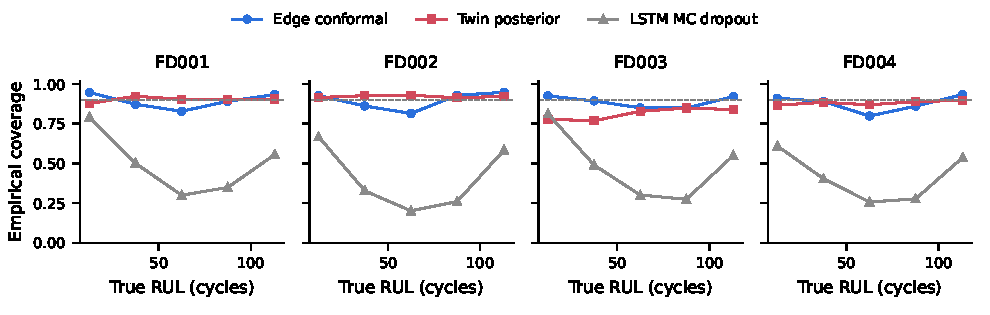
\includegraphics[width=\textwidth]{figures/coverage_horizon.pdf}
\caption{Empirical coverage of nominal 90\% intervals (dashed line) by true RUL, over all replayed cycles.}\label{fig:coverage}
\end{figure}

\subsection{Maintenance decisions}
Table~\ref{tab:decisions} reports Protocol B outcomes at the default threshold $\tau_g = 10$. Run to failure costs 40--48 per thousand cycles. Optimal age replacement cuts this to 8.1--8.7, but still lets 8 of 709 engines fail and leaves 79--116 cycles of life unused per engine. Every condition-based policy beats age replacement on cost, but those acting on point estimates are not safe: twin point fails 61 engines in total, LSTM point 23 and edge point 17, concentrated on FD004. Calibrated single-source bounds reduce failures to 6 (LSTM MC), 2 (edge conformal) and 2 (twin only). The hybrid policy is the only one with zero failures on every dataset. It reduces cost rate by 37\%, 34\%, 45\% and 47\% relative to age replacement and consults the twin on 21--28\% of cycles. At this threshold it is also the most conservative policy, leaving 20--28 cycles unused per engine, so its cost rate is 5--8\% above the oracle's.

\begin{table}[t]
\caption{Protocol B at $\tau_g = 10$: engines failed and cost rate $R\times 10^3$ per policy. The last two rows give the hybrid policy's mean unused life per preventively maintained engine (cycles) and its twin synchronization rate.}\label{tab:decisions}
\begin{tabular*}{\textwidth}{@{\extracolsep\fill}lcccccccc}
\toprule
& \multicolumn{2}{c}{FD001 (100)} & \multicolumn{2}{c}{FD002 (260)} & \multicolumn{2}{c}{FD003 (100)} & \multicolumn{2}{c}{FD004 (249)} \\
\cmidrule{2-3}\cmidrule{4-5}\cmidrule{6-7}\cmidrule{8-9}
Policy & Fail & $R$ & Fail & $R$ & Fail & $R$ & Fail & $R$ \\
\midrule
Run to failure      & 100 & 48.47 & 260 & 48.36 & 100 & 40.45 & 249 & 40.65 \\
Age replacement     & 1 & 8.49 & 1 & 8.13 & 2 & 8.12 & 4 & 8.69 \\
Oracle              & 0 & 5.09 & 0 & 5.08 & 0 & 4.22 & 0 & 4.24 \\
\midrule
Edge point          & 0 & 5.09 & 2 & 5.44 & 1 & 4.59 & 14 & 6.43 \\
Edge conformal      & 0 & 5.28 & 0 & 5.31 & 0 & 4.35 & 2 & 4.81 \\
LSTM point          & 0 & 5.08 & 0 & 5.08 & 1 & 4.60 & 22 & 7.61 \\
LSTM MC dropout     & 0 & 5.26 & 0 & 5.24 & 0 & 4.36 & 6 & 5.30 \\
Twin point          & 8 & 8.67 & 5 & 5.94 & 15 & 9.91 & 33 & 9.33 \\
Twin only ($q_{0.05}$) & 0 & 5.29 & 0 & 5.32 & 2 & 5.23 & 0 & 4.52 \\
\textbf{Hybrid}     & \textbf{0} & 5.36 & \textbf{0} & 5.39 & \textbf{0} & 4.48 & \textbf{0} & 4.58 \\
\midrule
Hybrid unused life & \multicolumn{2}{c}{19.6} & \multicolumn{2}{c}{21.2} & \multicolumn{2}{c}{23.7} & \multicolumn{2}{c}{27.8} \\
Hybrid twin sync rate & \multicolumn{2}{c}{0.280} & \multicolumn{2}{c}{0.265} & \multicolumn{2}{c}{0.221} & \multicolumn{2}{c}{0.214} \\
\botrule
\end{tabular*}
\end{table}

Fig.~\ref{fig:replay} shows one replayed engine. The edge estimate is noisy far from failure and its conformal band is wide. The twin's posterior narrows as observations accumulate and tracks the true trajectory closely once degradation begins. Synchronizations are sparse while the engine is healthy and become continuous once the edge estimate drops below 60, so the twin is consulted when its belief matters for the decision.

\begin{figure}[t]
\centering
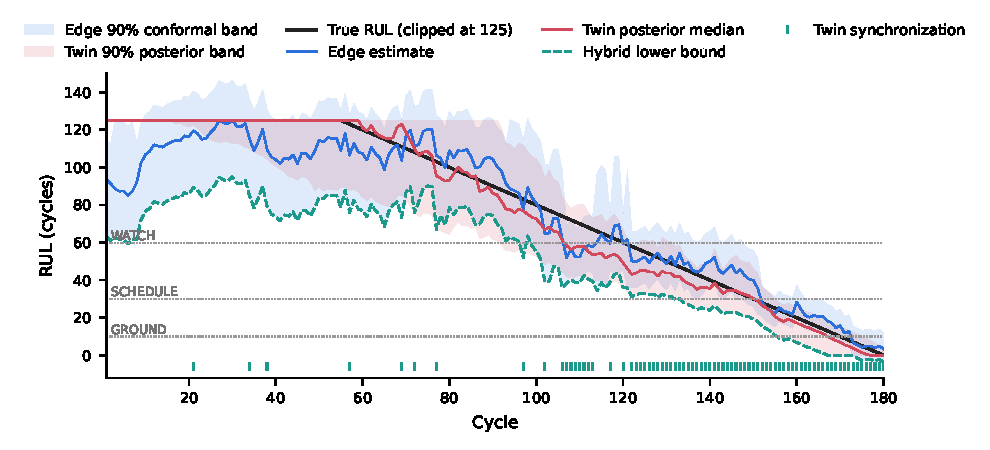
\includegraphics[width=\textwidth]{figures/engine_replay.pdf}
\caption{Replay of FD001 engine 14, held out in the first cross-validation fold. Shaded bands are 90\% intervals; ticks at the bottom mark cycles on which the twin was synchronized; dotted lines are the action thresholds.}\label{fig:replay}
\end{figure}

\subsection{Safety margin and threshold sensitivity}
A threshold of $\tau_g = 10$ builds a safety margin into every policy. To separate the quality of the bound from the size of the margin, we swept $\tau_g \in \{0, 2, 5, 10, 15, 20, 25, 30\}$ (Fig.~\ref{fig:sweep}). The hybrid policy has zero failures at every threshold on every dataset. Every other policy needs a positive margin somewhere: Table~\ref{tab:safe} lists, for each policy, the smallest threshold that was failure-free and the cost at the cheapest failure-free threshold. These thresholds were selected in hindsight on the replay itself, which favors the baselines.

With no margin ($\tau_g = 0$), the hybrid's cost rate is 5.07, 5.10, 4.26 and 4.38 per thousand cycles, which is 37--50\% below age replacement and within 3.3\% of the oracle. Even against baselines tuned in hindsight, its cost is the lowest on FD004 and within 0.4\% of the lowest on the other three sets. The practical difference is that the hybrid needs no tuning: it remains safe across the whole range of thresholds, whereas the safe threshold for the other policies differs by dataset and is not known in advance.

\begin{figure}[t]
\centering
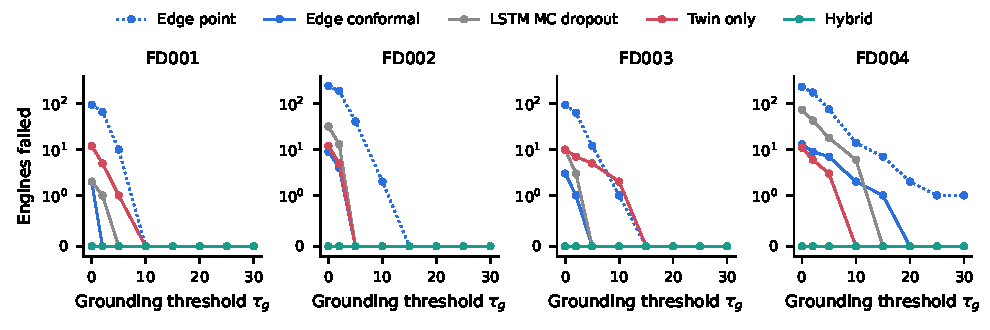
\includegraphics[width=\textwidth]{figures/threshold_sweep.pdf}
\caption{Engines failed versus grounding threshold $\tau_g$ (symmetric log scale). The hybrid policy is failure-free at every threshold.}\label{fig:sweep}
\end{figure}

\begin{table}[t]
\caption{Smallest failure-free grounding threshold $\tau_g$ in the sweep and cost rate $R\times10^3$ at the cheapest failure-free threshold. ``--'': no threshold in the sweep was failure-free.}\label{tab:safe}
\begin{tabular*}{\textwidth}{@{\extracolsep\fill}lcccccccc}
\toprule
& \multicolumn{2}{c}{FD001} & \multicolumn{2}{c}{FD002} & \multicolumn{2}{c}{FD003} & \multicolumn{2}{c}{FD004} \\
\cmidrule{2-3}\cmidrule{4-5}\cmidrule{6-7}\cmidrule{8-9}
Policy & $\tau_g$ & $R$ & $\tau_g$ & $R$ & $\tau_g$ & $R$ & $\tau_g$ & $R$ \\
\midrule
Edge point      & 10 & 5.09 & 15 & 5.23 & 15 & 4.30 & -- & -- \\
Edge conformal  & 2  & 5.06 & 5  & 5.16 & 5  & 4.25 & 20 & 4.91 \\
LSTM point      & 10 & 5.08 & 10 & 5.08 & 15 & 4.31 & 20 & 4.44 \\
LSTM MC dropout & 5  & 5.13 & 5  & 5.10 & 5  & 4.26 & 15 & 4.47 \\
Twin point      & 20 & 5.30 & 15 & 5.19 & 25 & 4.50 & 25 & 4.52 \\
Twin only       & 10 & 5.29 & 5  & 5.18 & 15 & 4.54 & 10 & 4.52 \\
\textbf{Hybrid} & \textbf{0} & 5.07 & \textbf{0} & 5.10 & \textbf{0} & 4.26 & \textbf{0} & \textbf{4.38} \\
\botrule
\end{tabular*}
\end{table}

\subsection{Ablations}
\paragraph{Fusion rule.} Replacing $\min(q_{0.05}, \ell^{e})$ with the twin's $q_{0.05}$ alone at synchronized cycles is safe at $\tau_g = 10$ on three sets but fails 2 engines on FD003; at $\tau_g = 2$ it fails 5, 5, 7 and 6 engines, and at $\tau_g = 0$ it fails 12, 12, 10 and 11. Min-fusion fails none in any of these settings. Near failure the twin's lower quantile can lag a sudden deterioration that the edge model sees within a window, and the minimum takes whichever bound reacts first.

\paragraph{Triggers.} Table~\ref{tab:triggers} removes or isolates each trigger at $\tau_g = 2$, where differences appear. The low-RUL trigger alone is sufficient for zero failures and accounts for most synchronizations; removing it causes failures on FD002 and FD004 even though the other two triggers remain. Sharp-drop and periodic triggers alone are cheap (5--8\% of cycles) but unsafe. In these data the sharp-drop and periodic triggers add synchronizations without changing any decision. They act as insurance for faults whose onset is not reflected in a low edge estimate, which C-MAPSS does not exercise.

\begin{table}[t]
\caption{Trigger ablation at $\tau_g = 2$: engines failed / twin synchronization rate.}\label{tab:triggers}
\begin{tabular*}{\textwidth}{@{\extracolsep\fill}lcccc}
\toprule
Triggers enabled & FD001 & FD002 & FD003 & FD004 \\
\midrule
All three             & 0 / 0.311 & 0 / 0.298 & 0 / 0.251 & 0 / 0.242 \\
Without low RUL       & 0 / 0.090 & 2 / 0.099 & 0 / 0.079 & 2 / 0.093 \\
Without sharp drop    & 0 / 0.280 & 0 / 0.261 & 0 / 0.229 & 0 / 0.210 \\
Without periodic      & 0 / 0.292 & 0 / 0.280 & 0 / 0.224 & 0 / 0.217 \\
Low RUL only          & 0 / 0.245 & 0 / 0.227 & 0 / 0.192 & 0 / 0.172 \\
Sharp drop only       & 0 / 0.064 & 4 / 0.076 & 1 / 0.046 & 3 / 0.064 \\
Periodic only         & 0 / 0.053 & 2 / 0.053 & 0 / 0.052 & 3 / 0.052 \\
\botrule
\end{tabular*}
\end{table}

\paragraph{Resynchronization period.} Varying the periodic trigger from 5 to 80 cycles, or disabling it, changes the synchronization rate (for example from 41\% to 29\% on FD001) but leaves every decision and cost unchanged, because lazy assimilation means a late synchronization loses no information.

\paragraph{Regime normalization.} With global instead of per-regime standardization on the multi-regime sets, edge RMSE degrades from 13.98 to 17.95 on FD002 and from 14.98 to 18.99 on FD004. The twin is far less sensitive (10.33 to 10.73 on FD002; 14.78 to 14.69 on FD004), because the learned HI weights partly absorb regime offsets.

\subsection{Computational cost}
The edge model is 150 trees and about 0.66--0.70\,MB serialized; one prediction is about 900 node comparisons plus 4.3--5.8\,k floating-point operations for the window summary, and takes 1.1--2.1\,ms single-threaded in Python on a commodity laptop. The LSTM needs 0.64--0.68\,M multiply--accumulates per pass and 12.8--13.7\,M for 20 MC-dropout passes. The twin holds 8000 floats of state per engine and costs about 24\,k floating-point operations per assimilated observation; a synchronization that ingests 20 buffered observations takes 1.8--2.6\,ms. At a 21--28\% synchronization rate, the hybrid consults the twin roughly one cycle in four, and between syncs the edge device transmits nothing.

%% ===================================================================== 7
\section{Discussion and limitations}\label{sec:discussion}

The results support three observations. First, last-cycle RMSE is a poor proxy for decision quality. On FD002 the LSTM point policy has the same cost as the oracle at $\tau_g = 10$, yet on FD004 it fails 22 engines; on FD001 the twin has worse benchmark RMSE than the edge model, yet it is the more accurate model over full trajectories. Second, calibrated lower bounds are what make a policy safe. Every point-estimate policy fails engines somewhere, and among bound-based policies the failures track the coverage results of Table~\ref{tab:coverage}. Third, two calibrated sources fused cautiously are safer than either alone, and the cost of that caution can be recovered by lowering the grounding threshold, which no single-source policy tolerates.

Several limitations apply. C-MAPSS is simulated, and real engines have maintenance histories, sensor faults and censored lifetimes that it does not model. The run-to-failure study uses cross-validation over training engines because the official test trajectories are truncated, so held-out engines come from the same simulation campaign as the training engines. The 10:1 failure-to-preventive cost ratio is an assumption, and the relative ranking of policies may change at other ratios. Conformal guarantees assume exchangeability, which windows from the same engine do not strictly satisfy; coverage was therefore checked empirically rather than assumed. The exponential HI model with a single threshold is least faithful on the two-fault-mode sets, which shows in FD003 coverage and the FD004 PHM08 score; a mixture over fault modes is a natural extension. Latencies were measured in Python on a laptop rather than on embedded hardware, so the operation counts are the more portable comparison. Finally, all results use one seed per fold; variance across seeds was not measured.

%% ===================================================================== 8
\section{Conclusion}\label{sec:conclusion}

This paper presented Twin Turbo, a hybrid framework in which a conformally calibrated edge model runs every cycle and a per-engine particle-filter digital twin is synchronized only when a trigger fires, and evaluated it on the maintenance decisions it drives rather than on last-cycle error alone. The twin is competitive with published deep models on the official C-MAPSS test sets and better calibrated than MC dropout. Replaying 709 engines to failure, the hybrid policy prevented every failure, cut the long-run cost rate by 34--47\% relative to optimal age replacement, consulted the twin on about a quarter of cycles, and was the only policy that stayed failure-free at every grounding threshold. Future work will extend the twin to multiple fault modes, study sensitivity to the cost ratio, and validate the approach on field data and embedded hardware.

\backmatter

\bmhead{Acknowledgements}
The authors thank NASA's Prognostics Center of Excellence for making the C-MAPSS data publicly available.

\section*{Declarations}

\begin{itemize}
\item \textbf{Funding:} No funding was received for conducting this study.
\item \textbf{Conflict of interest:} The authors have no competing interests to declare that are relevant to the content of this article.
\item \textbf{Ethics approval and consent to participate:} Not applicable.
\item \textbf{Consent for publication:} Not applicable.
\item \textbf{Data availability:} The C-MAPSS turbofan degradation dataset is publicly available from the NASA Prognostics Center of Excellence data repository.
\item \textbf{Materials availability:} Not applicable.
\item \textbf{Code availability:} The source code, experiment scripts and cached results are available at \repourl.
\item \textbf{Author contribution:} Archit Singh: conceptualization, methodology, software (digital twin, hybrid decision layer and evaluation framework), formal analysis, writing -- original draft, project administration. Vedant Vadke: software (data pipeline and edge model), validation, investigation. Rishabh Raushan: software (LSTM baseline and interactive replay console), visualization, data curation. Sreevarsh Mahesh Gandhi: investigation (literature review), validation, writing -- review and editing. All authors read and approved the final manuscript.
\end{itemize}

\bibliography{references}

\end{document}
